\section{Universal Verification Methodology Multi-Language}\label{uvm_ml}

\begin{figure}[htb]
 \centering
 %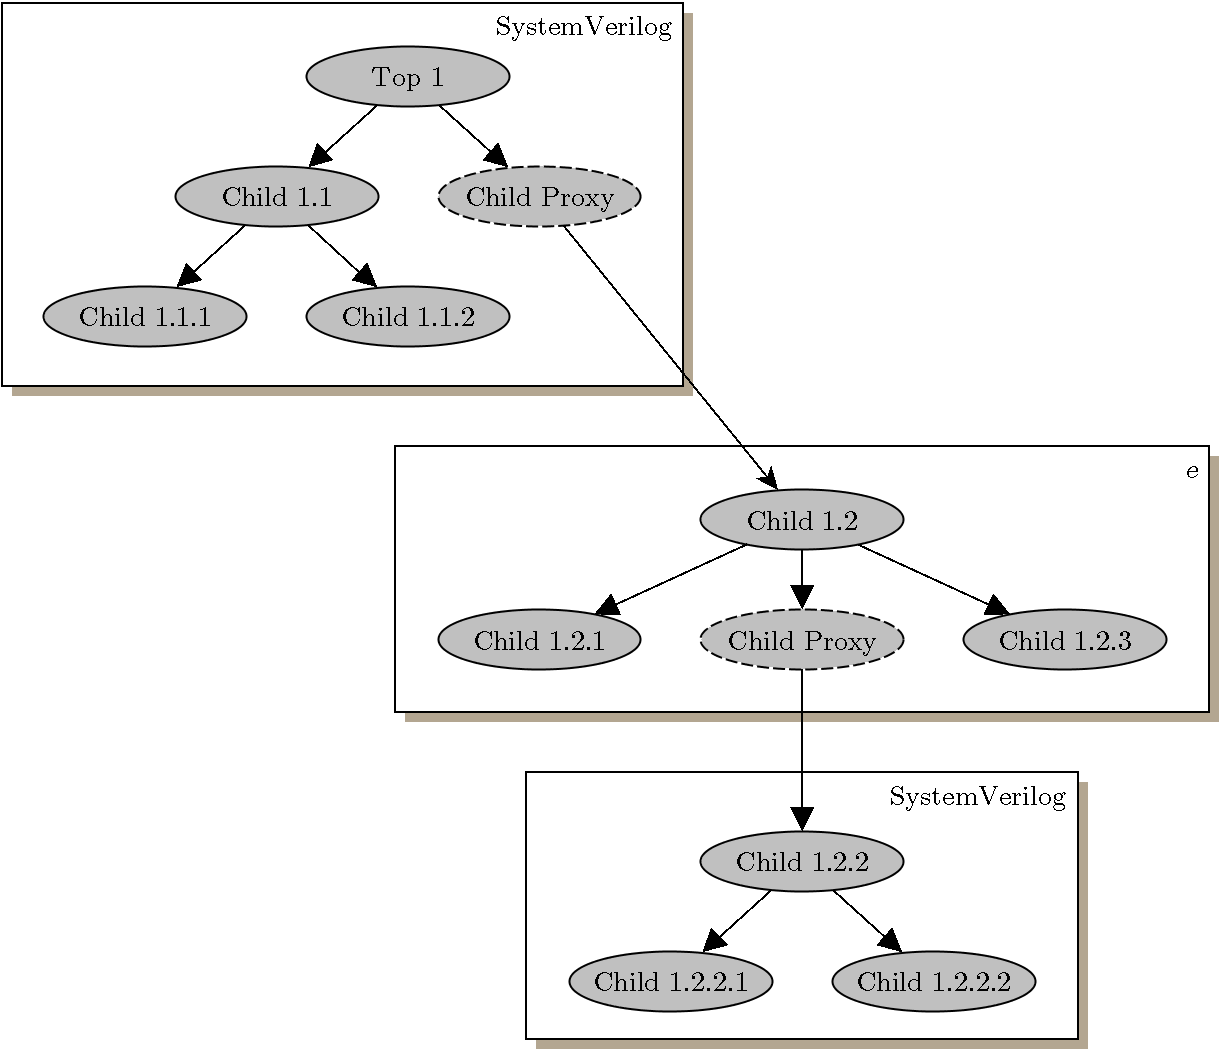
\includegraphics[width=1.0\textwidth,angle=0]{abb/UVM_ML_unified}
 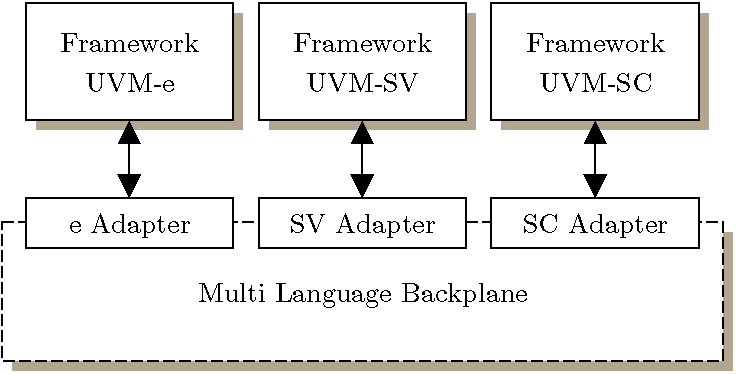
\includegraphics[scale=0.3]{abb/UVM_ML_architecture}
 \caption{UVM-ML architecture}
\label{fig:UVM_ML_architecture}
\end{figure}

\subsection{Integrate Multi-Language Functionality into Incisive Enterprise
Simulator}
- where to get UVM-ML\\
- how to install\\
- problems with installation\\
\\
\subsection{Creating a Multi-Language Environment}
A verification environment typically consists of a system UVC containing
multiple subsystem UVCs, interface UVCs or module UVCs. These are composed in a
hierarchical way. With UVM-ML an environment can be constructed with components,
which are implemented in different frameworks. For example it could be composed
of an interface UVC implemented in UVM-SV and a module UVC in
UVM-\textit{e}. \\
When planing to create such a multi-language environment, there
are two possible approaches supported by UVM-ML to achieve this goal. Firstly an
\emph{unified hierarchy} can be created or alternatively an \emph{side-by-side}
environment. In an unified hierarchy a child component implemented in one
verification language is instantiated from a parent component in another
verification language. In contrast, when creating a side-by-side architecture,
the environment contains multiple tops.

\subsubsection{Creating an \emph{Unified Hierarchy} Environment}
To implement an \emph{unified hierarchy} each component which instantiates a
component of another framework needs to create and connect a proxy to
this component (this can be seen in figure~\ref{fig:UVM_ML_unified}). Then the
backplane applies operations which are performed on the proxy to the
corresponding component in the other verification language. This gives the
opportunity to use some of UVM-ML's benefits. It is possible to use a predefined
phasing in this environment. Where phases like build, connect or run are
performed depth-first to ensure that dependencies between the components of
different frameworks are resolved in the right way. Also sub components can be
configured which increases the reusability of the environment, because when the
environment is included in some other environment, only the top component needs
to be configured and all sub components are configured automatically. Because of
this it is recommended to implement such an environment.\\
Following it is described how to create a \emph{unified hierachy} which
instantiates a SystemVerilog component within an \textit{e} unit and vice versa.

\begin{figure}[htb]
 \centering
 %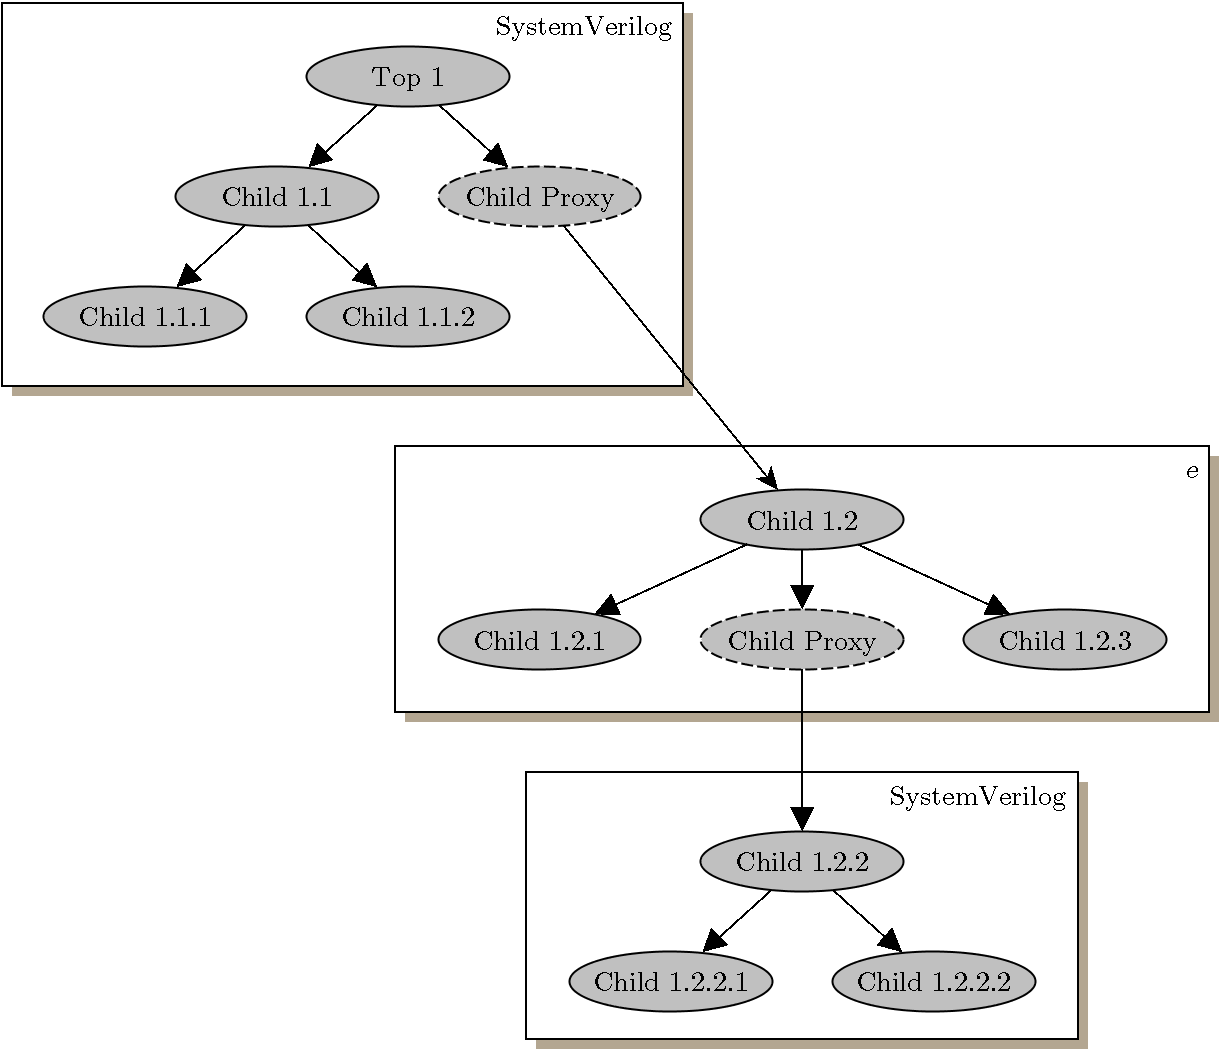
\includegraphics[width=1.0\textwidth,angle=0]{abb/UVM_ML_unified}
 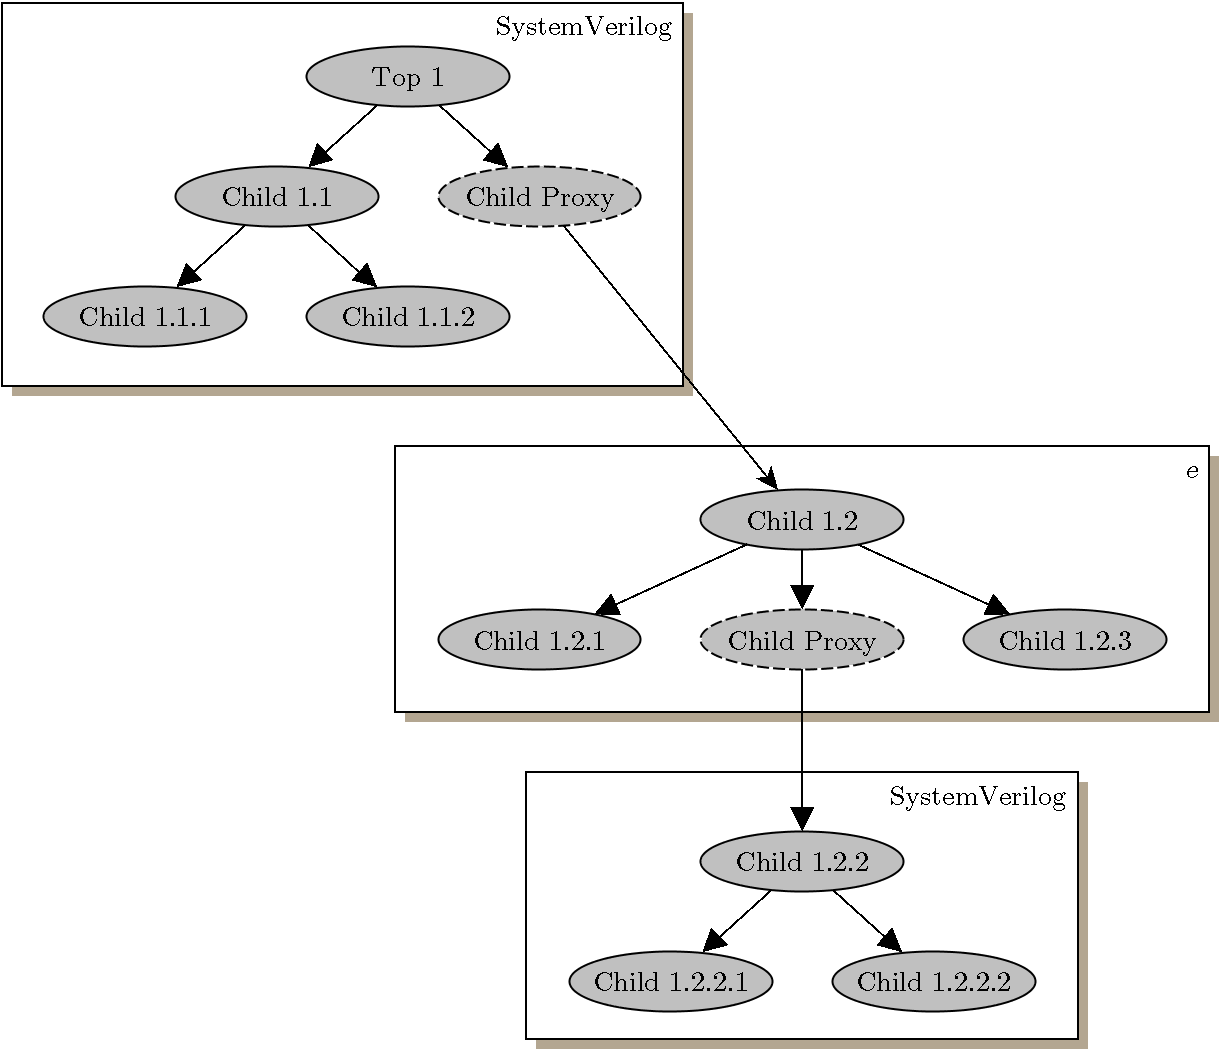
\includegraphics[scale=0.3]{abb/UVM_ML_unified}
 \caption{Structure of an \emph{unified hierarchy} environment}
\label{fig:UVM_ML_unified}
\end{figure}

\paragraph{Instantiating a SystemVerilog Component within an \textit{e} Unit}
\label{sv_inside_e}
When instantiating a SystemVerilog component within an \textit{e} unit,
it is necessary to instantiate a proxy unit inside the \textit{e} unit. After that the
proxy unit and the SystemVerilog component need to be connected. \\
An example for the code of the extended SystemVerilog component can be seen in
listing~\ref{lst:SV_unified_sub}).
It is recommended to extend the SystemVerilog component
(line~\ref{line_extend_component}) which will
be reused and then put all multi-language functionalities inside this new
component to ensure that the original component can still be used in
non-multi-language environments. The extended one needs to include the UVM
package (line~\ref{line_uvm_package}/\ref{line_uvm_macros}) as well as the adapter
package for SystemVerilog (line~\ref{line_uvm_ml_package}).
After that all additional multi-language functionalities can be put inside the
class like configuring this sub component (see section~\ref{ml_config}) or data
communication via TLM ports (see section~\ref{ml_tlm}).
\medskip
\lstset{language={SystemVerilog}, escapechar=|}
\begin{lstlisting}[frame=htrbl, caption={SystemVerilog code example: extended
component}, label={lst:SV_unified_sub}]
import uvm_pkg::*;					|\label{line_uvm_package}|
`include "uvm_macros.svh"			|\label{line_uvm_macros}|
import uvm_ml::*;					|\label{line_uvm_ml_package}|

class ml_ubus_env extends ubus_env;			|\label{line_extend_component}|
  `uvm_component_utils(ml_ubus_env)
  function void build_phase(uvm_phase phase);
    // Additional multi-language functionalities
  endfunction : build_phase
endclass : ml_ubus_env
\end{lstlisting}
\medskip
Corresponding to the extensions in the SystemVerilog component the \textit{e}
unit needs to include an proxy unit for it(see listing~\ref{lst:e_unified_top}).
This can be done by instantiating an unit of type
\lstinline$child_component_proxy$ (line~\ref{line_uvm_ml_e_proxy}) which is a
predefined datatype in \textit{e}.
Through constraining the proxy unit's \lstinline$type_name$ field
(line~\ref{line_uvm_ml_e_proxy_keep}) the
SystemVerilog component is integrated into the hierarchy. Thereby the string
needs to be composed of \lstinline$target_frmw_indicator:component_type_name$, where
\lstinline$target_frmw_indicator$ (case-insensitive) identifies the framework
of the instantiated foreign child component and can be \lstinline$SV$ for
UVM-SystemVerilog, \lstinline$e$ for UVM-\textit{e} or \lstinline$SC$ for UVM-SystemC and
\lstinline$component_type_name$ is the type of the instantiated component.
\medskip
\lstset{language=e, escapechar=|}
\begin{lstlisting}[frame=htrbl, caption={\textit{e} code example:
instantiating the SystemVerilog component in the \textit{e} unit},
label={lst:e_unified_top}]
unit ubus_env {
  uvc_top: child_component_proxy is instance;	|\label{line_uvm_ml_e_proxy}|
    keep uvc_top.type_name =|\,\,|= "SV:ml_ubus_env";|\label{line_uvm_ml_e_proxy_keep}| 
};
\end{lstlisting}

\paragraph{Instantiating an \textit{e} Unit Within a SystemVerilog Component}
When reusing an \textit{e} unit inside of an SystemVerilog component it is
necessary to integrate an proxy for the e unit within the SystemVerilog
component and then connect both.\\
As shown in listing~\ref{lst:SV_unified_top} this proxy component is created by
declaring an component of type \lstinline$uvm_component$ inside the parent
component (line~\ref{line_sv_declare_proxy}). In the \lstinline$build_phase$ this proxy component is
instantiated via calling \lstinline$uvm_ml_create_component$ (line~\ref{line_sv_create_proxy}) with the following
syntax:
\medskip
\lstset{language={}, numbers=none, escapechar=|}
\begin{lstlisting}
function uvm_ml::child_component_proxy uvm_ml_create_component(
  string target_frmw_indicator,
  string component_type_name,
  string instance_name,
  uvm_component parent=null)
\end{lstlisting} 
\medskip
Where \lstinline$target_frmw_indicator$ indicates the framework adapter of the
foreign component (see section~\ref{sv_inside_e}),
\lstinline$component_type_name$ is the type of the foreign component according
to its declaration inside its framework, \lstinline$instance_name$ is the name
of the instance of the component proxy and \lstinline$parent$ is the handle of
the parent instance (\lstinline$this$ indicates the current component).\\
Because multi-language functionality is already integrated in UVM-\textit{e}, the child unit does not need any changes
to support the creation of an \emph{unified hierarchy} environment.
\medskip
\lstset{language=SystemVerilog, numbers = left, escapechar=|, breaklines=true}
\begin{lstlisting}[frame=htrbl, caption={SystemVerilog code example:
instantiating an e unit}, label={lst:SV_unified_top}]
class testbench extends uvm_env;
  uvm_component xbus_uvc;|\label{line_sv_declare_proxy}|
  `uvm_component_utils(testbench)

  function void build_phase(uvm_phase phase);
    super.build_phase(phase);
    xbus_uvc = uvm_ml_create_component("e", "xbus_env_u", "xbus_uvc", this); |\label{line_sv_create_proxy}|
  endfunction
endclass : testbench
\end{lstlisting}

\subsubsection{Creating a \emph{Side-by-Side} Environment}

When there is no need for creating an \emph{unified hierarchy} environment, UVM-ML supports also the ability to build an
environment with multipe tops as can be seen in figure~\ref{fig:UVM_ML_side_by_side}. Here each tree inside of an
framework has its root instantiated as top component. This architecture is called \emph{side-by-side} and best
applicable when there is only limited synchronization required between the components of different frameworks. This is
indicated by the limitations of the architecture. It is not possible to use multi-language configuration as described in
section~\ref{ml_config}. Additionaly the behavior of the phase execution is limited. Here each phase is first executed
completely on one tree before moving on to the next one. 

\begin{figure}[htb]
 \centering
 %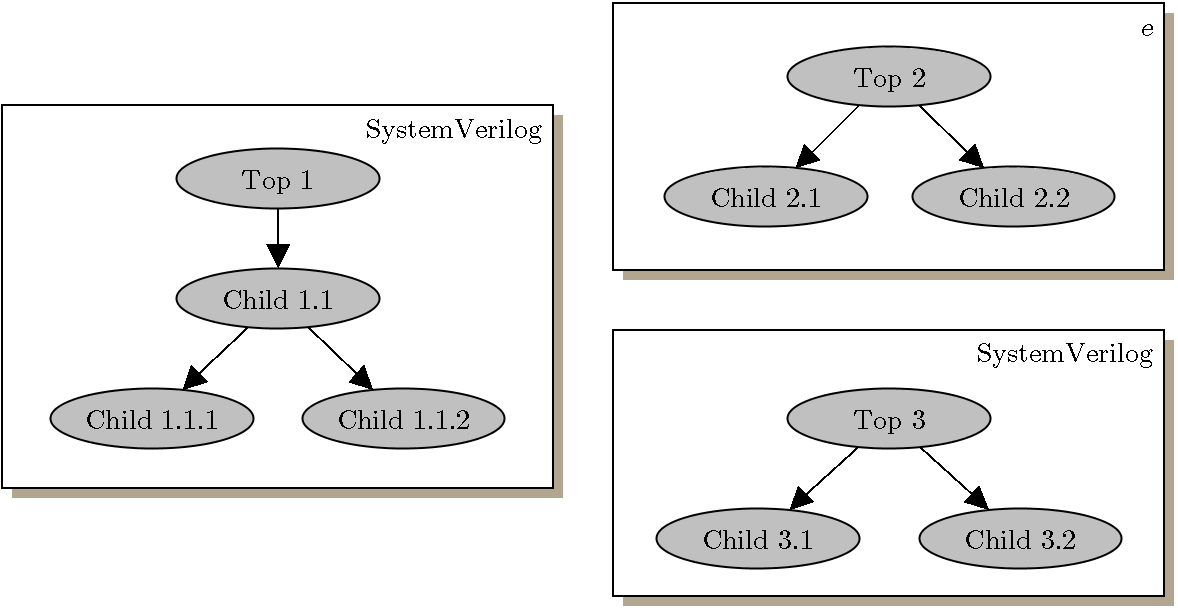
\includegraphics[width=1.0\textwidth,angle=0]{abb/UVM_ML_side_by_side}
 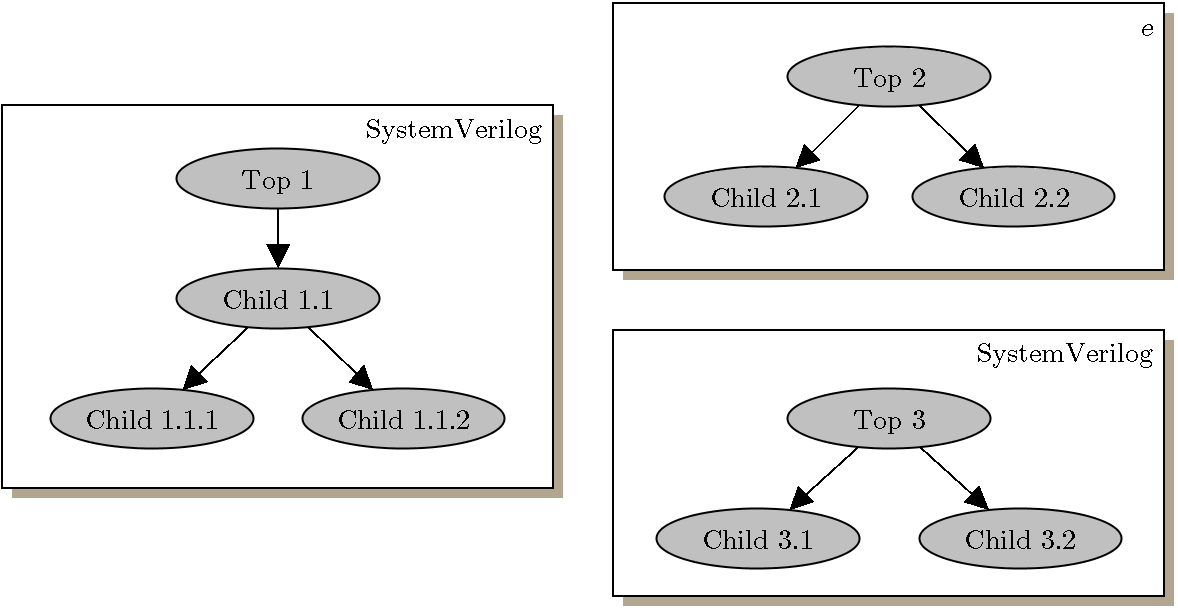
\includegraphics[scale=0.3]{abb/UVM_ML_side_by_side}
 \caption{Structure of an \emph{side-by-side} environment}
\label{fig:UVM_ML_side_by_side}
\end{figure}

\subsection{Configuring a Multi-Language Environment} \label{ml_config}

After building a multi-language environment its often necessary to perform additional configurations before starting a
test run. For example, setting an agent as passive respectively active or the number of resources available. In an
environment with an \emph{unified hierarchy} such configurations can be propagated from one framework tree
to all sub-trees in other frameworks. This is achieved by using the native UVM configuration constructs of each
framework, which are listed below:
\begin{itemize}
\item{UVM-SystemVerilog:}
%\medskip
\lstset{language={}, numbers=none, escapechar=|}
\begin{lstlisting}
uvm_config_db#(T)::set()
uvm_config_db#(T)::get()
\end{lstlisting} 
%\medskip

\item{UVM-\textit{e}}
%\medskip
\lstset{language={}, numbers=none, escapechar=|}
\begin{lstlisting}
keep uvm_config_set()
keep uvm_config_get()
\end{lstlisting} 
%\medskip
\end{itemize}

Each framework maintains its own configuration database. These are synchronized automatically via the multi-language
backplane when a configuration is set. Thereby for getting the configuration information each framework just needs to
access its local database.



\subsection{Data Communication in a Multi-Language Environment} \label{ml_tlm}
- tlm-port e -> sv\\
- tlm-port sv -> e\\
- type mapping\\
\\
\subsection{Sequence Layering in a Multi-Language Environment}
- adding tlm interface\\
- create proxy sequencer\\
- doing sequence items\\
- doing sequences\\

\subsection{Running an Multi-Language Environment with Incisive Enterprise Simulator}

After completing the testbench the final step is to run the multi-language environment. Here is shown how to achieve
this with Incisive Enterprise Simulator (IES) provided by Cadence Design Systems Inc. Also a task of the
UVM-SystemVerilog adapter is presented for this purpose, which provides an alternative option for running a testbench.

\subsubsection{Setup IES for UVM-ML Mode}

\subsubsection{Starting a test with the irun utility} \label{uvm_top}

IES provides command line switches for its \lstinline$irun$ utility to declare the top component(s) of the testbench as
well as the test to be started as shown below.
\medskip
\lstset{language={}, numbers=none, escapechar=|}
\begin{lstlisting}
-uvmtest frmw_indicator:test_name
-uvmtop frmw_indicator:top_name
\end{lstlisting} 
\medskip
Both \lstinline$uvmtest$ as well as \lstinline$uvmtop$ firstly need to identify the framework adapter of the test
respectively top component. This is done via \lstinline$frmw_indicator$ which can be \lstinline$SV$, \lstinline$e$ or
\lstinline$SC$ as described in section~\ref{sv_inside_e}. Seperated via a colon comes the actual test/top component. For
UVM-\textit{e} this is the full path of the file containing it. In contrast UVM-SystemVerilog along with UVM-SystemC use
its component type name. So contrary to UVM-\textit{e} the full path to the file containing it has to be forwarded to
\lstinline$irun$ prior to that.

\subsubsection{Starting a test via the UVM-SystemVerilog adapter}

Alternativly to these command line switches the UVM-SystemVerilog adapter supports a procedure call to set the top
component(s) respectively the test of the multi-language testbench. The other adapters for UVM-\textit{e} and
UVM-SystemC do not support such a call. So there is the only possibility to use the above mentioned command line
switches. The task provided by the UVM-SystemVerilog adapter is called \lstinline$uvm_ml_run_test$ and has the following
syntax:
\medskip
\lstset{language={}, numbers=none, escapechar=|}
\begin{lstlisting}
task uvm_ml_run_test(
  string tops[],
  [string test = ""])
\end{lstlisting} 
\medskip
Where \lstinline$tops[]$ is a dynamic array of top component identifiers and \lstinline$test$ represents a
SystemVerilog or SystemC test component or the full path of an file containing an \textit{e} test unit. Both arguments
support the same syntax as the command line switches to specify the components (see section~\ref{uvm_top}). The argument
indicating the test component is optional for the purpose of just generating the multi-language environment.
